\documentclass[11pt]{report}
\usepackage{cs1200}
\usepackage{graphicx}
\usepackage{float}
\usepackage{xcolor}

\begin{document}

\psHeader{3}{Thu Feb. 26, 2026 (11:59pm)}

Please see the syllabus for the full collaboration and generative AI policy, as well as information on grading, late days, and revisions.

All sources of ideas, including (but not restricted to) any collaborators, AI tools, people outside of the course, websites, ARC tutors, and textbooks other than Hesterberg--Vadhan must be listed on your submitted homework along with a brief description of how they influenced your work. You need not cite core course resources, which are lectures, the Hesterberg--Vadhan textbook, sections, SREs, problem sets and solutions sets from earlier in the semester. If you use any concepts, terminology, or problem-solving approaches not covered in the course material by that point in the semester, you must describe the source of that idea. If you credit an AI tool for a particular idea, then you should also provide a primary source that corroborates it. Github Copilot and similar tools should be turned off when working on programming assignments.

If you did not have any collaborators or external resources, please write 'none.' Please remember to select pages when you submit on Gradescope. A problem set on the border between two letter grades cannot be rounded up if pages are not selected OR collaborators not noted.

\textbf{Your name: Joaquin de Castro}

\textbf{Collaborators and External Resources: I asked Yara a couple minor questions, such as on putting continue after goto case to avoid the +=1.}

\textbf{No. of late days used on previous psets: 0}

\textbf{No. of late days used after including this pset: 1}

\vspace{1em}
The purpose of this problem set is to solidify your understanding of the RAM model (and variants), and the relations between the RAM model, the Word-RAM model, Python programs, and variants. In particular, you will build skills in simulating one computational model by another and in evaluating the runtime of the simulations (both in theory and in practice).


\begin{enumerate}

    \item (Simulation in practice: RAMs on Python)
    In the Github repository, we have given you a partially written Python implementation of a universal RAM Model simulator.  Your task is to fill in the missing parts of the code to obtain a complete universal RAM simulator.
     Your simulator should take as input a RAM Program $P$ and an input $x$, and simulate the execution of $P$ on $x$, and return whatever output $P$ produces (if it halts).  The RAM Program $P$ is given as a Python list $[v,C_0,C_1,\ldots,C_{\ell-1}]$, where $v$ is the number of variables used by $P$.  For simplicity, we assume that the variables are named $0,\ldots,v-1$ (rather than having names like ``tmpptr'' and ``insertvalue''), but you can introduce constants to give names to the variables.  The $0$\textsuperscript{th} variable will always be $\inputlen$, the $1$\textsuperscript{st} variable $\outputpointer$, and the $2$\textsuperscript{nd} variable $\outputlen$.  A command $C$ is given in the form of a list of the form $[\cmd]$, $[\cmd,i]$, $[\cmd,i,j]$, or $[\cmd,i,j,k]$, where $\cmd$ is the name of the command and $i,j,k$ are the indices of the variables or line numbers used in the command.  For example,  the command $\var_i = M[\var_j]$ would be represented as $(\READ,i,j)$.  See the Github repository for the precise syntax as well as some RAM programs you can use to test your simulator.

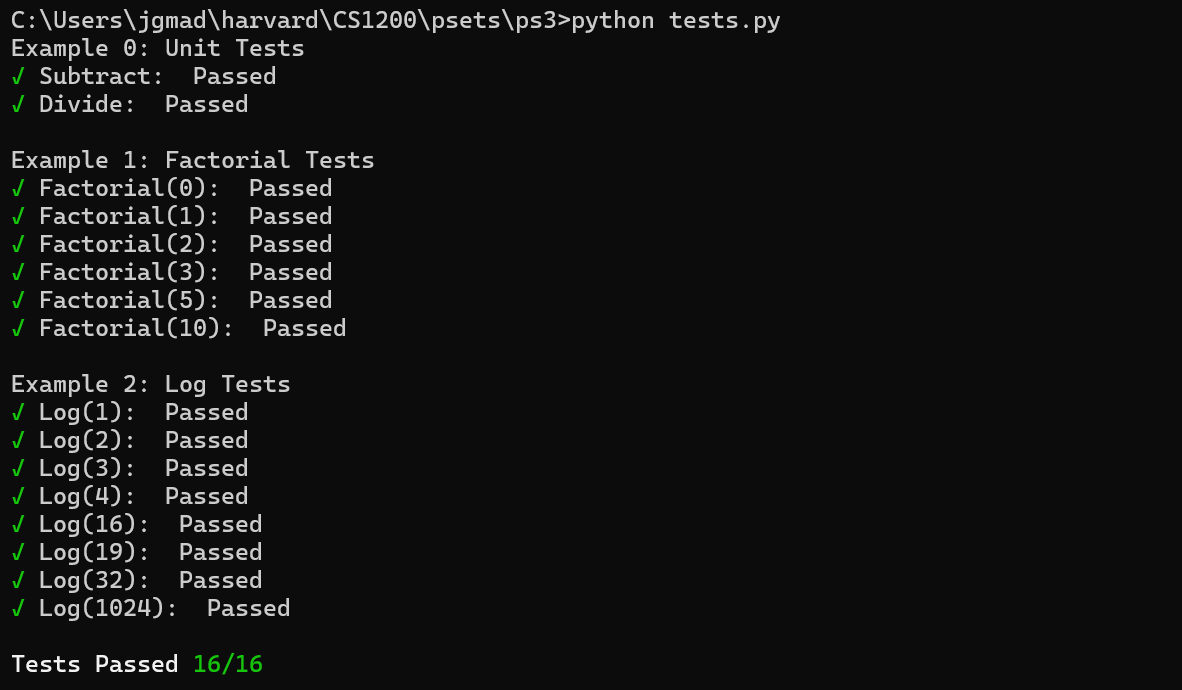
\includegraphics{image.png}

\item (Empirically evaluating simulation runtimes and explaining them theoretically)

Consider the following two RAM programs:

\begin{algorithm}[H]
\Input{A single natural number $N$ (as an array of length 1)}
\Output{$14^{2^N+1}$ (as an array of length 1)}
\Variables{$\inputlen, \outputpointer, \outputlen, \counter, \result$}
\setcounter{AlgoLine}{-1}
$\zero = 0$\;
$\one = 1$\;
$\fourteen = 14$\;
$\outputlen = 1$\;
$\outputpointer = 0$\;
$\result = 14$\;
$\counter = M[\zero]$\;
\Indp
 IF $\counter == 0$ GOTO \ref{line:done}\; \label{line:loop}
$\result = \result \times \result$\;
$\counter = \counter - \one$\;
IF $\zero == 0$ GOTO \ref{line:loop}\;
\Indm
$\result = \result \times $\fourteen\; \label{line:done}
$M[\outputpointer]=\result$\;
\end{algorithm}

\begin{algorithm}[H]
\Input{A single natural number $N$ (as an array of length 1)}
\Output{$14^{2^N+1} \bmod 2^{32}$ (as an array of length 1)}
\Variables{$\inputlen, \outputpointer, \outputlen, \counter, \result, \temp, \W$}
\setcounter{AlgoLine}{-1}
$\zero = 0$\;
$\one = 1$\;
$\fourteen = 14$\;
$\outputlen = 1$\;
$\outputpointer = 0$\;
$\result = 14$\;
$\W = 2^{32}$\;
$\counter = M[\zero]$\;
\Indp
IF $\counter == 0$ GOTO \ref{line:done2}\; \label{line:loop2}
$\result = \result \times \result$\;
$\temp = \result / \W$\;
$\temp = \temp \times \W$\;
$\result = \result - \temp$\;
$\counter = \counter - \one$\;
IF $\zero == 0$ GOTO \ref{line:loop2}\;
\Indm
$\result = \result \times \fourteen$\; \label{line:done2}
$\temp = \result / \W$\;
$\temp = \temp \times \W$\;
$\result = \result - \temp$\;
$M[\outputpointer]=\result$\;
\end{algorithm}


\begin{enumerate}
    \item Exactly calculate (without asymptotic notation) the RAM-model running times of the above algorithms as a function of $N$.
    Which one is faster? \label{itm:RAMtime}

    {\color{blue}{

    First Program:
        
    Lines 0 to 5 are all assignments which are 1 time step = 6.

    At line 6, we now have a loop of N iterations. This is because we start at counter = M[0] = N, and at each run through lines 6 to 10 we decrease the counter by exactly 1. Within each loop, we have 4 lines.

    Following this loop, the goto line that sees the counter as 0 adds a time step, and then lines 11 and 12 are now each just one time step as they are primitive operations.

    In total, this is thus $7+4N+1+2 = 4N+9$

    Second Program:

    Lines 0 to 7 are assignment operators which gives 8
    We have a similar loop in lines 8 to 14 which gives 7N
    The last goto that sends the program to line 15 is one time step, and then Lines 15-19 are each one time step which gives 5
    Answer: $ 8+7N+1+3 = 7N+14$

    From here, we can see that the first program is theoretically faster.
    }}
    \item Using your RAM Simulator, run both RAM programs on inputs $N=0,1,2,\ldots,15$ and graph the actual running times (in clock time, not RAM steps).  (We have provided you with some timing and graphing code in the Github repository.) Which one is faster?  \label{itm:realtime}
    
    \color{blue}{Here program 1 actually seems to take longer than program 2; program 1 appears to run in exponential time, indicating that perhaps one or more of the operations we took for granted in program 1 is/are not actually one time step.}
    \item Explain the discrepancies you see between Parts~\ref{itm:RAMtime} and \ref{itm:realtime}.  (Hint: What do we know about the relationship between the RAM and Word-RAM models, and why is it relevant to how efficiently the Python simulation runs?)

    \color{blue}{Word-RAM models indicate the memory register have a restricted size or word length. A Python implementation is in reality more closely or accurately modeled by a word RAM model because we have finite memory. In particular, if our word length limit is $2^{32}$}, then operations that have results taking up space more than the word length size, then we can no longer assume that the operation takes O(1) time. Since Program 2 essentially takes the result of the multiplication step mod $2^{32}$ in each iteration, we do not expect to drastically exceed the word length, which from research appears to be $2^{32}$ or $2^{64}$. 
    \color{blue}{My guess at this point is that since the result variable in Program 1 exponentially increases, the time steps to account for the overflow in the word length may also increase with each iteration, which results in the exponential as opposed to linear growth.}
    \item (optional\footnote{This problem won't make a difference between N, L, R-, and R grades.}) Give a theoretical explanation of the shapes of the runtime curves you see in Part~\ref{itm:realtime}, by providing explicit formulas for the asymptotic runtimes of the two programs (in clock time). You may need to do some research online and/or make guesses about how Python operations are implemented to come up with your estimates.

\end{enumerate}

\item (Simulating Word-RAM by RAM)
For every Word-RAM program $P$, there is a RAM program $R$ that simulates $P$ in the following sense.  For every $n \in \N$, input array $x$ of length $n$, word-length $w$, and time bound $t$, $R(x,2^w, \max_i x[i],t)$ should do the following:
\begin{itemize}
    \item If $P[w](x)$ halts without crashing within $t$ steps, then $R$ should halt with the same as the output of $P[w](x)$.
    \item If $P[w](x)$ crashes or fails to halt within its first $t$ steps, then the $R$ should indicate so by halting with $\outputpointer=\outputlen=2^w$.
    \item The runtime of $R$ should be $O(t)$ and the largest memory location accessed by $R$ should be at most $n+t$.
    \item All of the values that $R$'s variables and memory cells hold during the computation should have bitlength at most $O(w+\log \max_i x[i] + \log n)$.
\end{itemize}
Your proof should use an {\em implementation-level} description, similar to the proof that RAM programs can be simulated by ones with at most $c$ registers in Theorem 6.4 from the Hesterberg-Vadhan textbook.

Recall that Word-RAM programs have a finite but changing memory size $S$; you may want to start your simulation by initializing $S$.  Then think about how each operation of a Word-RAM program $P$ can be simulated in a RAM program $R$, taking care of any differences between their semantics in the Word-RAM model vs. the RAM model. Don't forget MALLOC!

Your proof should use an {\em implementation-level} description, similar to the proof that RAM programs can be simulated by ones with at most $c$ registers in Theorem 6.4 from the Hesterberg-Vadhan textbook. Your answer should include - at least - the following aspects:
\begin{itemize}
\item Initialization: How the memory in the RAM program R will be initialized? Be mindful of the additional "default variables" that a Word-RAM program has, in comparison to the RAM program. Recall that Word-RAM programs have a finite but changing memory size $S$; you may want to start your simulation by initializing $S$.

\textcolor{blue}{We note that a word-RAM particularly differs from a RAM model in that it is initialized with two additional parameters, the word length w and memory S. We can write these two to registers as variables w and S, where we set S to n. This only takes O(1) time. Already in the RAM program we know that the input array x is already encoded in initialization into memory locations 0 to n-1. We also have that we have a variable $input_len set$ to n.}

\textcolor{blue}{Additionally, if any $x[i] > 2^w-1$ where $x\in [n]$, then we set $output_ptr = output_len = 2^w$ and goto the end of the program (halt)}

\textcolor{blue}{Lastly, if $n>2^2$ then set $output_ptr = output_len = 2^w$ and goto the end of the program (halt).}

\item Operations: For each operation in the Word-RAM program P, how will the corresponding operation in the RAM program R be performed? Keep in mind that the RAM program "may not by default know" of nuances of the arithmetic in Word-RAM.

\textcolor{blue}{Division and subtraction in the simulating RAM program are defined in the same way as the word-RAM program. However, for multiplication and addition, if the output exceeds or is equal to $2^{w}$, we set the result of either to be $2^w - 1$.}

\textcolor{blue}{Assignment commands: If a command in P that R is simulating assigns to a variable or writes to memory a number that is greater than or equal to $2^w$, then we set $output_ptr = output_len = 2^w$ and goto the end of the program (halt). Whenever we assign to memory at index i, we always check $i-S$ and if this is 0 we do nothing, otherwise we proceed with assignment.}

\textcolor{blue}{Malloc: We implement Malloc in RAM by increasing the variable S by 1. If the new value of the variable S is 0, we set $output_ptr = output_len = 2^w$ and goto the end of the program (halt).}

\textcolor{blue}{There are t steps and at most t of those steps can be malloc steps. Because of how we define assignment, we only write to memory if we have incremented S sufficiently by a prior malloc step. Thus we will never write to memory beyond memory location n+t.}

\textcolor{blue}{Importantly, for each of the changes we have made to the original RAM operations, we have at most increased them by O(1) runtime. For our malloc implementation, this also primarily just involves incrementing S by 1 or addition, which also remains to be O(1)}

\item Memory: How will the read and write into the memory locations take place? Keep in mind that the RAM program "may not by default know" of nuances of memory reads or writes in the Word-RAM.

\textcolor{blue}{Malloc: We implement Malloc in RAM by increasing the variable S by 1. If the new value of the variable S is 0, we set $output_ptr = output_len = 2^w$ and goto the end of the program (halt).}

\textcolor{blue}{For writing to memory, if we want to write to an index i, we check $i-S=0$ using goto and if so then set $output_ptr = output_len = 2^w$ and goto the end of the program (halt).}

\textcolor{blue}{For reading to memory, if we want to read an index i, we check $i-S=0$ using goto and if so then set $output_ptr = output_len = 2^w$ and goto the end of the program (halt).}

\item Output: How will the output of the Word-RAM program P be simulated in R? Again, keep the differences between Word-RAM and RAM program in mind.

\textcolor{blue}{If we have not set $output_ptr = output_len = 2^w$ and goto the end of the program (halt), meaning the program has not crashed, and if it did this part would be skipped anyway, following all of the operations we can now write the output to memory}

\textcolor{blue}{However, our output will only be from $M[output_len]$ to $M[min(output_ptr+output_len-1,S-1)]$}

\item Runtime: Justify how your simulation maintains the runtime stated above.

\textcolor{blue}{Importantly, for each of the changes we have made to the original RAM operations, we have at most increased them by O(1) runtime. For our malloc implementation, this also primarily just involves incrementing S by 1 or addition, which also remains to be O(1)}

\textcolor{blue}{Our runtime is thus just a constant plus our original runtime for P, which is O(c+t) = O(t)}

\item Bitlength: justify how your simulation maintains the bitlength stated above.

\textcolor{blue}{In big O notation, our maximum bitlength is just the maximum of the log of the size we allowed when writing to memory, which is $2^w$, the maximum element in our input array we had which is $max_ix[i]$, and of course the input length variable which is n. In big O notation since we just care about the upper bound we can take the log of each these then add them together.}

\item Don't forget MALLOC and updates to the GOTO command!

\textcolor{blue}{For the goto command, if any variable that is involved exceeds the allowed bitlength as set by w, then we set $output_ptr = output_len = 2^w$ and goto the end of the program (halt)}

\end{itemize}

\item (reflection) In what ways do LLMs impact your learning outcomes for this course? If you use LLMs in learning course material, give some example(s) of how they helped you learn something that lectures/sections etc did not. If you do not use LLMs, discuss reasons for why you do not use them. All opinions are valid.

Quick note on grading: Good responses are usually about a paragraph, with something like 7 or 8 sentences. Most importantly, please make sure your answer is specific to this class and your experiences in it. If your answer could have been edited lightly to apply to another class at Harvard, points will be taken off.

\textit{Note: As with the previous psets, you may include your answer in your PDF submission, but the answer should ultimately go into a separate Gradescope submission form.}

\item Once you're done with this problem set, please fill out \href{https://forms.gle/7U7bXytpVMCRzbZ8A}{this survey} so that we can gather students' thoughts on the problem set, and the class in general. It's not required, but we really appreciate all responses!

\end{enumerate}

\end{document}